%%%%%%%%%%%%%%%%%%%%%%%%%%%%%%%%%%%%%%%%%%%%%%%%%%%%%%%%%%%%%%%%%%% 
%                                                                 %
%                             Animation                           %
%                                                                 %
%%%%%%%%%%%%%%%%%%%%%%%%%%%%%%%%%%%%%%%%%%%%%%%%%%%%%%%%%%%%%%%%%%% 
 
\chapter{ANIMATION}
\label{chapter:animation}

Jumping is the acceleration of a character's center of mass upward.  Acceleration is applied in excess and in opposition to gravity, resulting in the character breaking contact with the ground and traveling a short distance before contact is re-established.  This acceleration results due to the character pushing against the ground, first bending

Jumping motions can be divided into several stages.  First is the lead-up or wind-up stage in which the character flexes, preparing their muscles for contraction and providing space for their body to extend.  This takes the form of a slight crouch.  Next comes the thrust stage, in which the character extends and exerts a force against the ground to accelerate upward.  The character pushes against the floor with their feet, the contractions of the muscles causing joints to unbend and as a result displace the character's center of mass causing work to be done.  This extension and resulting thrust is caused by the contraction of muscles, which produce torques on the skeleton.

Once the character has broken contact with the ground, they travel through the air, their velocity decreasing steadily due to gravity, air resistance, and other forces until they eventually land.  Once they regain contact with the ground, the character absorbs or disperses the kinetic energy of their jump.

We attempted two main approaches to producing a jump motion through muscle simulation.  The first method focused heavily on the torques produced by the muscles, but ultimately failed due to unknown reasons.  The second method focused on the kinetic energy and performed calculations to match the energy of the muscles, which simplifies the movement and produced a successful simulation.

\section{Setup and Inputs}
The character in our system consists of a mesh, a skeleton, and a controller which has itself several sub-components.  First we constructed a mesh, a 3D visual representation of our character.  Our mesh is a simple, blocky humanoid, lacking arms in order to focus more heavily on the lower body motion of the figure.  A more complex human character, or even a humanoid non-human character could be substituted.  This mesh consists of vertices, which each have a position as well as other information not relevant to our simulation such as normal and texture coordinate, which are used by \unity for displaying the mesh.  This mesh can also be referred to as a character model, but in the context of this simulation we will refer to it as the mesh.  Three vertices form a triangular face, though these are often created as quadrilaterals by the artist as the topology of the model can be simpler to work with due to the grid patterns formed as compared to triangular meshes.  In the case of quad meshes, the mesh is often treated as a triangle mesh by the game engine or renderer, with each quad producing two triangles.

Our mesh was created using \maya, positioning the vertices in groups or individually, using several rectangular prisms as a base.  Using the edge loop tool, more vertices were inserted, with loops of edges circling the torso and legs to produce the final shape.  This mesh was then rigged, meaning a skeleton was added.  As described in further detail in \ref{subsection:skel_joints}, joints were positioned individually relative to the mesh, attempting to mimic the positioning of joints in the human skeleton.  The connections were made simply, with each joint acting as a ball and socket joint, meaning that constraints needed to be specified at a later stage to facilitate hinge joints such as the knee and ankle and that complex, multi-boned structures as found in the foot and shin were simplified to a single bone connecting two joints.  The hierarchy of joints for the skeleton was rooted at the pelvis with three children: one leading to the upper body and one to each hip.  From there a single joint was used for the manipulation of the upper body, with separate joints for each hip, knee, ankle, toe, and heel.  Though there is no movement in the toe, placing a bone for the foot requires an end joint for the bone to connect to.

%TODO how do i talk about this with authority, there isn't really anything to cite there's just youtube videos and it's generally taught as such/discovered via industry
% found some articles, gamasutra especially
Joints are then associated with the mesh through weight painting, in which each vertex of the mesh is assigned a weight for each joint.  This weight designates if and how much a vertex transforms when a joint is moved.  Each vertex must be assigned a weight for each joint of the model.  Careful weight assignment is highly important as this determines the behavior of the character's ``skin'' when they move, affecting how the mesh twists or bends as well as which parts move with which bones.  The joints may then be used to manipulate the mesh to produce animations, with each keyframe in an animation storing information about each joint instead of each vertex.

\subsection{User Specified Constants}
\label{subsection:user_constants}
% specified constants
% gravity
% air time
% windup time
% error allowance (between calculated skeleton values and desired)
% drag
% jumping policy (not implemented)
% Windup PD k values
% Balance PD k values
% muscle values foreach muscle:
%	k (linear spring constant)
%	anchor joints (for our simulation, 2)
% 	center joint
%   [0,1] scale to indicate muscle anchor position (0 is closer to center joint, 1 is closer to end joint)
%   bone width
% calculated values
Within the controller there are a number of constants the user can specify, outside of the character itself.  These specify constants for the simulation environment as well as some constants describing the animation to be produced.  Our only environmental constant is gravity, which we specify as -10 $\frac{m}{s^2}$, where the negative indicates the downward direction.  Other constants include the air time, windup time, error allowance, and constants for the PID controllers which specify a multiplicative factor for the proportional, integral, and derivative components of each PID controller.

The times indicate how much time the character is expected to spend in the air and winding up for the jump.  Air time in our case consists of the portion of the animation where the character's feet are not in contact with the ground plane.  Windup time refers to the time in which the character has their feet on the ground and is in the process of accelerating their mass upwards as the initial takeoff portion of the jump.  A long windup time gives a very slow, exaggerated jumping motion while a short windup gives a very rapid, clipped motion.  While we allow the user to specify any time for both air and windup, in practice there is a limited range of values that are possible for the character.  Values outside of the reasonable range produce indeterminate or strange behaviors in the simulation, such as either failing to find a muscle load that can feasibly produce the jump or attempting to produce the jump and failing partway.
%TODO figure of failed jumps due to bad time selection
\begin{figure}[ht]
	\centering
	\caption{Examples of jumps with poorly selected times.}
	\label{fig:bad_time_jumps}
\end{figure}

%TODO table of values from testing excel sheet showing why it fails
\begin{table}[ht]
	\centering
	\caption{Values for calculated necessary velocity given air and windup times for a skeleton with muscle k values around 200000.}
\end{table}

Error allowance in our simulation is a widely used value indicating a percent error tolerance.  This tolerance is used for determining the allowable difference between the desired values of either resultant linear acceleration and desired acceleration for the torque based simulation, or calculated kinetic energy and total elastic energy for the energy based simulation.  The allowable difference is used for choosing samples and determining if the character has satisfied either the energy or acceleration requirements to complete the windup stage.  The same error allowance is also used to determine if the limb usage is greater than a minimum to complete the windup stage, which is used to force a degree of bend in extreme cases, where very little bend is required as the muscles are extremely strong or the jump distance is very small.  This minimum is applied to compensate for the contraction rates of muscles, which would require a higher degree of bend than our muscle model does, leading to a more realistic simulation.  Below is an example of the inequality using the error allowance.

\[
	E_{kinetic} - E_{elastic} \le \epsilon E_{kinetic}
\]

Lastly, we utilize proportional-integral-derivative (PID) controllers, which require 3 constants for each controller.  A PID controller modifies an input based on error in 3 ways: proportional to the error, proportional to the integral of the error, and proportional to the derivative of the error.  This allows changes to the system to have gains directly related to the error through the proportional component, eliminate steady-state error with the integral component, and to adjust gain with the derivative to improve stability of the changes.  Our system does not require an integral component, meaning our controllers are just PD controllers with their constant for I set to 0.  For our controllers, as we work in discrete frames, our controller calculation is as follows.
\[
	u(t) = k_p e(t) + k_i \displaystyle\sum_{\tau = 0}^t e(\tau) + k_d \left( e(t) - e(t-1) \right)
\]

%TODO example windup times with our chosen values

\subsection{Skeleton, Joints, and Muscles}
\label{subsection:skel_joints}

\begin{figure}[ht]
	\centering
	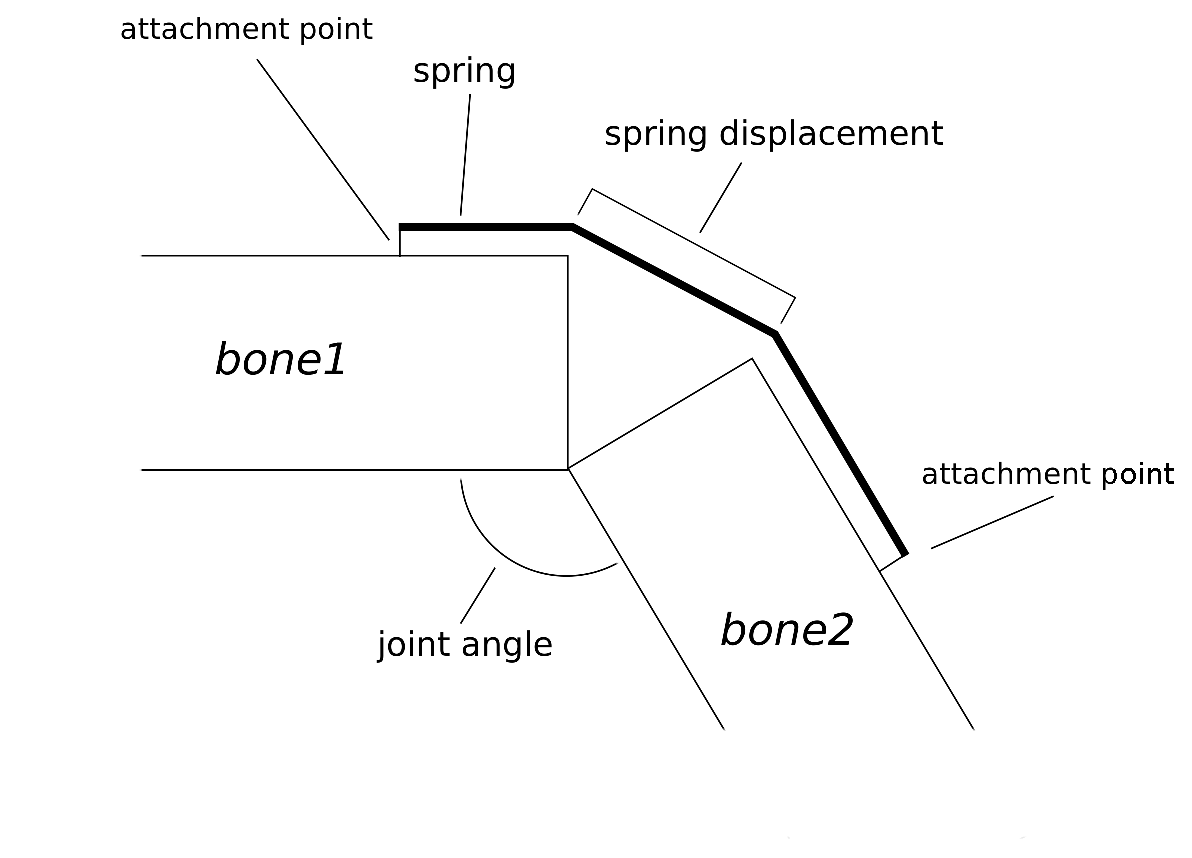
\includegraphics[width=10cm]{images/spring_calc/spring_angle_calc.eps}
	\caption[Diagram of muscle setup]{Visual representation of the setup of bones and muscles for a single joint.  This illustrates the method by which we calculate the spring displacement, taking the bones as rigid blocks which separate and stretch the string as the joint bends.}
	\label{fig:forceCalc}
\end{figure}

For the purposes of animation, a joint is an object with an associated position, associated transformation, a parent joint, and some number of child joints.  In the case of the root, the parent joint is absent and in the case of the end joints such as tips of the fingers there are no child joints.  Each child joint is connected to the parent by a rigid bone, which protrudes from the parent at a given resting angle.  These joints are structured in a tree, as the parent and child joints imply, with the root of the tree at the pelvis.  This tree serves as a hierarchy for transformations.

Joints are associated with a set of vertices from the mesh to be animated.  Each of these may be associated with multiple joints, and are assigned a weight for each joint which acts as a scale factor for the transformations performed on the vertex.  When a joint is transformed, the transformation is propagated to the children, with the parent as the origin of the child node's coordinate system.

In addition to the animation related functions, joints in our system handle a number of other functions and values.  Each joint keeps track of its constraints on rotation.  Rotations are performed axis-angle, which makes the constraints somewhat more complicated.  Constraints are specified through euler angles: pitch, roll, and yaw.  These correspond to a rotation about the x, z, and y axes respectively in \unity's coordinate system.  When rotating using a traditional rotation matrix through Euler angles, constraints simply prevent any of the angles from exceeding the bounds.  The other issue was how to constrain a joint when rotation about a certain axis was fully prohibited, such as the knee joint which can only rotate about the x-axis.  To constrain the axis-angle rotation thus, simply zero the undesirable component of the vector.  Constraining the axis-angle rotation to a region with degree minima and maxima for rotations around the x, y, and z axes requires definition and constraint to the region of a sphere the rotation constraints covers.  Instead of solving this complex problem, we instead clamp the euler angles to their constrained regions after each rotation.

Along with constraints, each joint tracks a weight, which allows distribution of weight over the body.  This distribution affected the torque simulation heavily as the torque of each joint resulted in a different angular momentum depending on the mass distribution.  The energy simulation considered the character as a rigid body, not considering the changes occurring due to weight distribution except for balance issues and the effects on the muscles as described shortly.  Joints also provide functions for calculating the direction to the next joint for muscle calculations, and a utility function for returning to a resting position.

Several joints form a muscle.  Though any number of joints is possible, our muscles only utilize 3 joints each.  These joints serve as anchor points, as seen in \cite{muscle_based_bipeds}.  The muscle itself is a linear spring, obeying Hooke's law.  This gives force ($F$) and elastic energy ($E_{elastic}$) as
\begin{align*}
	F &= -ks \\
	E &= \frac{1}{2} k s^2
\end{align*}\
where $k$ is the spring constant for the muscle and $s$ is the displacement of the spring.  The negation of $k$ in the force calculation indicates the force restores the spring to rest.

Considering a muscle as a spring models a muscle at maximum activation.  A relaxed muscle has very little contractual or restoring force, and thus a low value for $k$, while a flexed muscle has a large $k$.  While the muscle model could take muscle activation level into account, we chose the simpler system, allowing the user to specify $k$ for their particular case.  This gives more control for the animation, but also allows for more errors and issues.  The results with poorly chosen $k$ values resemble the results with poorly chosen times.

\begin{figure}[ht]
	\centering
	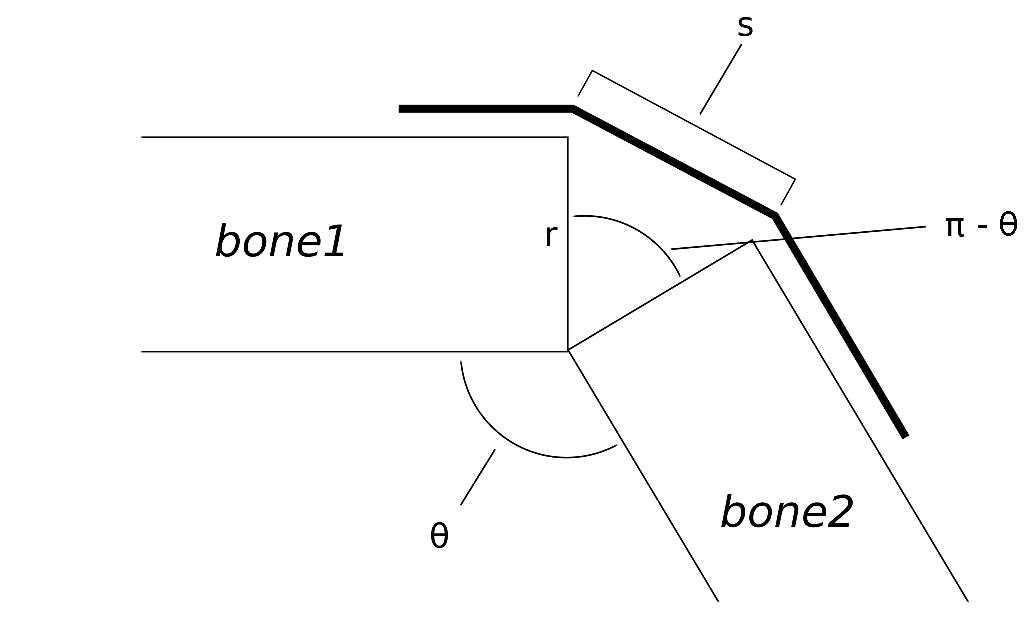
\includegraphics[width=10cm]{images/spring_calc/angle_diag.eps}
	\caption[Diagram of spring displacement calculation]{Above is a visual representation of the angles used to calculate the spring displacement.  The angle of the joint, $\theta$, is used to calculate the displacement $s$ using the bone width $r$ and the law of sines.}
	\label{fig:angleDiag}
\end{figure}

Along with the $s$ values, a muscle keeps track of its center joint, anchor joints, and the bone width.  A muscle has two anchor points and crosses the center joint.  The positions of the anchors are specified as values in the range $[0,1]$ along the bone between the center joint and the anchors.  Bones are considered to be rectangular prisms with a square cross-section, with a width $r$ specified by the user.  Spring displacement can then be calculated directly from the angle of the joint using these constants and our assumptions as illustrated in Figure \ref{fig:forceCalc} with the equation below derived from the law of sines:
\[ 
	s = \dfrac{r\sin\left(\pi - \theta \right)}{\sin\frac{\theta}{2}}
\]
We derive this equation by calculating the supplementary angle, opposite the spring displacement.  This angle can therefore be expressed as $\pi - \theta$. The sum of the remaining angles of the triangle formed by the spring displacement and bone ends can then be expressed as $\frac{\theta}{2}$.  These angles are shown in Figure \ref{fig:angleDiag}. We assume uniform bone width, which allows a simpler calculation of the angles.

For utility purposes we have each muscle calculate its utilization, giving a value in $[0,1]$.  This utilization is calculated as the dot product of the normalized vectors between the center joint and the anchor points.  The value is then scaled from $[-1, 1]$ to $[0,1]$ by adding 1 and dividing by 2.

\section{Center of Mass and Balance}
\label{section:com}
%TODO need to standardize usage of joint to anatomical, animation, or something else
The center of mass (CoM) is calculated as the centroid of the character.  More specifically, joint positions are averaged, with a weight assigned to each joint based on the weight of the limb associated.  The CoM must be recalculated with each update to the character's pose as the shift in weight changes the position.

Using the calculated CoM, the balance of the character can be determined by the position of the CoM relative to the supporting polygon of the character.  The supporting polygon is a polygon determined by the points of contact of the character with the ground or other supports which provide a normal force to counteract gravity and other external forces.  During the windup and thrust phases, the character maintains contact with the ground through their feet, with the outer edges of the feet forming two sides of a quad, a line between the two feet at the toes forming a third, and a line between the heels of the character forming the fourth side.  This polygon should be parallel to the ground plane, and is positioned at the bottom of the feet.  If the character's center of mass is over this supporting polygon, the character is balanced.

%\begin{figure}[ht]
%	\centering
%	\caption[Algorithm diagram for calculation of balance error]{Balance error calculation.}
%	\label{fig:balanceErr}
%\end{figure}

To quantify balance, the vector between the center of the supporting polygon and the position of the CoM is measured.  This vector is then projected into the same plane as the supporting polygon, giving a 2 dimensional error between where the CoM is currently and where it would need to be to be perfectly centered.  The PD controller then attempts to minimize the magnitude of this vector by moving in the proscribed direction while bending to achieve the desired force, constraining the number of solutions possible to provide the desired force.

% does the vertical distance have effect?  you're going to fall over more easily if you're on a stilt as opposed to crouching over your feet as the moment will be (bigger? is that bigger?).  the lever will be more able to move your weight easily

% upper body rebalancing
As the character bends for the windup and extends for thrusting, the character must rebalance without using its legs in order to maintain the calculated load on the muscles.  For these cases, the upper body is used to rebalance.  The character bends forwards, backwards, left, and right to shift the weight of the upper body to offset the balance error created by the lower body pose.  This is performed using a PD controller, with the error input as the balance error as calculated above, and the output as the amount to rotate in each direction subject to skeletal constraints.

\section{Inverse Kinematic Solving}
\label{section:ik}
As the skeleton is a hierarchy assumed to be rooted at the hip, a problem arises with applying rotations to joints.  To keep a character's feet rooted to the floor as is expected, positions must be solved for using inverse kinematics.  Given the desired position for the hip, and the desired position of the foot, the joint angles and positions of the knee and ankle are solved for.  Constraints are placed on each joint, limiting the range of motion to an expected range as well as limiting the axes about which each joint can rotate, preventing unnatural directions of motion.  These values are specified per joint and can be edited by the user to simulate varied levels of flexibility or alternate body shapes.

%TODO alternate body with digitigrade, Tauren or whatever from WoW, raptor style...
%TODO Further justification of why choosing this method instead of learning is that this is more user-tunable as opposed to a learning heavy model which doesn't allow as much user tuning

\begin{table}[ht]
	\centering
	\caption[Table of joint constraints]{Joint angle constraint values used for each joint, with accompanying images of expected motion range.}
	\label{tab:jointConstraints}
\end{table}

A solution to the joint positions is found greedily using these constraints, and gradient descent method which works on single-chains of joints.  A single chain of joints is a sequence of joints in which each joint has a single child and a single parent, with one root joint and one leaf joint which lack a parent and child respectively.  Given the hierarchy of joints and a desired position for one of the non-root nodes of the chain, cyclic-coordinate descent (CCD) is used to determine rotations of the joints between the joint in question and the root that will minimize the distance between the joint in question and the desired position.  This algorithm is shown in \ref{alg:ik}.

\begin{algorithm}[ht]
	\centering
	\begin{algorithmic}[H]
		\Function{SingleChainIK}{C, D, E}
		\Repeat
		\ForAll{Joints R between E and the root, starting with the end E}
			\State $\theta_R = \vec{RD} \times \vec{RE}$
		\EndFor
		\Until{\textit{Desired number of iterations performed} or \textbf{E} \textit{is close enough to} \textbf{D}}
		\EndFunction
	\end{algorithmic}
	\caption[Single chain IK algorithm]{Given chain of joints C, move joint E to position D using cyclic coordinate descent (TODO cite CCD references).  This process iteratively moves joint E closer to the location D, concentrating on each joint R in the chain one at a time and solving the geometric problem of minimizing distance between E and D by rotating R.}
	\label{alg:ik}
\end{algorithm}

This approach is simpler to implement than other approaches such as the pseudo-inverse of the Jacobian for the specific case of single chains of joints.  In addition, this approach allows some flexibility, specifically in constraints of the joints.  As each joint is addressed individually instead of the system as a whole, any constraints placed on the joint can easily be accounted for by simply preventing the joint from rotating out of the desired range while the rest of the system continues to move as close as possible to the solution.  One downside is that a halting condition must be determined, through a minimum acceptable distance.  To handle the case where the joint cannot be moved within this minimum distance, a maximum number of iterations must be designated.  In practice, 100 iterations is enough to converge, with as few as 30 working well for our simulation.

%%%%%%%%%%%%%%%%%%%%%%%%%%%%%%%%%%%%%%%%%%%%%%%
%               Torque Method                 %
%%%%%%%%%%%%%%%%%%%%%%%%%%%%%%%%%%%%%%%%%%%%%%%
\section{Torque-based simulation}
\label{section:torque}
One method of simulation we attempted used springs placed along the length of each limb to produce a torque on the joints of the character.  This method failed for unknown reasons.  Torques on the joints results from the force of the muscle pulling a bone to rotate about the joint, resulting in a complex system of motion with each bone rotating around the joints.  These rotations combine to move the body in a direction, allowing a character's control to be centered around degree and timing of muscle activation. Our method for this type of simulation was inspired by the other work in complex muscle based simulation for bipeds. \cite{muscle_based_bipeds}  In our case, we take the muscle as constantly activated, which means that its spring constant defines the strength of the muscle, allowing the user to set the activation manually.  This muscle is then stretched to produce the desired torque by bending the affected limb.  The restoring force of the spring-muscles produce torques which are used to calculate angular momentum, and from that linear momentum.  Linear momentum is then used to calculate the resulting acceleration.

\subsection{Path Estimation}
\label{subsection:torque_path}
%\begin{figure}[ht]
%	\centering
%	\begin{tikzpicture}[node distance=1cm and 1cm, auto]
% Path Estimate Phase
	%	Path Estimate Stage
    \node [stage] (path) {\nodebox{5cm}{Path Estimate \[a = \dfrac{2 (x - x_0 - v_0 t)}{t^2} \]}};
    %	Path Estimate Data
    \node [data, above= of path] (xf) {\nodebox{2cm}{Target Position ($x$)}};
    \node [data, left= of xf] (xi) {\nodebox{2cm}{Initial Position ($x_0$)}};
    \node [data, left= of xi](t) {\nodebox{2cm}{Time ($t$)}};
    \node [data, right= of xf] (vi) {\nodebox{2cm}{Initial Velocity ($v_0$)}};
    \node [data, below= of path] (accel) {\nodebox{3cm}{Target Acceleration ($a$)}};
    
    \path [line] (xi) |- (path);
    \path [line] (xf) -- (path);
    \path [line] (t) |- (path);
    \path [line] (vi) |- (path);
    \path [line] (path) -- (accel);
\end{tikzpicture}
%	\caption[Diagram of path estimation algorithm]{Diagram of the path estimation step.}
%	\label{fig:pathEstimate}
%\end{figure}

\begin{figure}[ht]
	\label{fig:pathExample}
	\caption[Example of estimated path]{Example of a path estimation.}
\end{figure}
Before calculations relating to the model's skeleton are performed, an initial estimate of the jump path is performed.  The estimate uses a forward kinematic calculation to determine the velocity required to move an object through the air from the initial position of the model to a final position.

The user specifies a desired time ($t_{air}$), which indicates the time the character will spend airborne during the animation, i.e. the time between when the character's feet break contact with the ground and when they regain contact with the ground.  This is useful as the desired animation can be more easily adjusted to fit a desired time as an in-game animation or to fit a particular storyboard for an animated film sequence.

The initial velocity is given by a manipulation of a simple kinematic equation \[ \vec{x} = \vec{x_0} + \vec{v_0} t_{air} + \frac{1}{2} \vec{a} t_{air}^2 \] derived from the relationships between acceleration ($\vec{a}$), velocity ($\vec{v}$), and displacement ($\vec{x} - \vec{x_0}$), namely
\begin{align*}
	\vec{v} &= \dfrac{d\vec{x}}{dt} \\
	\vec{a} &= \dfrac{d\vec{v}}{dt}
\end{align*}.

This relationship gives us the velocity, given a known start position ($\vec{x_0}$), destination ($\vec{x}$), acceleration ($\vec{a}$), and time ($t_{air}$).  As this describes the path of the character once it breaks contact with the ground, the time referred to only covers the time between the character breaking contact with the ground and when their feet touch again at the end of the jump  The only force, and therefore acceleration acting upon the character while in the air is gravity, thus giving 
\[ \vec{v_0} = \dfrac{\vec{x} - \vec{x_0}}{t_{air}} - \dfrac{\vec{g}t}{2} \]
to describe the initial velocity our character has upon breaking contact with the ground, which then decays over the course of the jump due to gravity to produce a parabolic path.  The equation considers the character as a point mass traveling in a vacuum, meaning there is no consideration of friction, drag, or rotational movements.  Acceleration can then be determined as 
\begin{align*}
	a &= \dfrac{dv}{dt} \\
	&= \dfrac{\vec{v_f} - \vec{v_i}}{t_{windup}} \\
	&= \dfrac{\vec{v_0} - {v_i}}{t_{windup}}
\end{align*}
where $\vec{v_i}$ is the initial velocity of the character before the jump calculations began.  This accommodates jumps where the character is already moving.

%There is an additional modification to the equation of $\frac{1}{2} g t_{air}$, which considers that the upward velocity of the acceleration is determined by gravity.  Assuming that gravity is a vector with only a vertical component, we can calculate the necessary vertical component for our acceleration by calculating the initial velocity achieved from our calculated acceleration by using the fact that $a = \dfrac{dv}{dt} = \dfrac{v - v_0}{t}$ or $v = v_0 + at$.  By calculating the velocity resulting from the windup, $v = at$ we can substitute this into 

\subsection{Windup}
\label{subsection:torque_windup}
%From this force, the acceleration can be determined using $F=ma$ from classical mechanics.  This assumes the character is a rigid body with negligible air resistance acted upon by gravity of $10\frac{m}{s}$.  The mass is calculated as the summed total of the distributed masses assigned to the character's limbs, which are summed to produce a total mass for the character.

Using the calculated velocity and acceleration, we compare the desired values to achieve a particular path with the values produced by the muscles on the skeleton.  To compute a resultant instant linear acceleration, we start from the muscle and calculate the torque resulting from the muscle's contraction.  First we calculate the scalar force of the muscle-spring as $F = -k s$ where $s$ is the spring displacement as calculated in \ref{subsection:skel_joints}.  Using the scalar force, we calculate the torque and the angular momentum.  Torque magnitude can be calculated as \[\tau = r F\] where $r$ in this case is the scalar distance between the pivot point and the location of force application.  In our case, this is the distance from the center of the joint to the major anchor point, which we consider to be the anchor point highest in the hierarchy, which is the bone most expected to move.  The direction of the torque is the normal vector to the plane of rotation, calculated as the cross product between the directions to each anchor point which gives the plane of rotation about the joint.

Angular momentum is derived from torque, as \[\vec{\tau} = \dfrac{d\vec{L}}{dt}\] where $\vec{\tau}$ is torque and $\vec{L}$ is the angular momentum.  The angular momentum can then be calculated as $\vec{\tau} t_{windup}$.  Angular momentum is used to calculate linear momentum by finding the tangent to the circle at the moment of takeoff.  The magnitude of the linear momentum is then calculated as \[p = \frac{L}{r}\] which then gives the acceleration as follows \[ \vec{a} = \frac{1}{m}\left(\dfrac{d\vec{p}}{dt}\right)\] where m is the mass of the character.

\subsubsection{Sampling}
\label{subsubsection:torque_sample}
In order to determine the position of the character that produces this acceleration, we sample uniformly over the region in which the character is balanced.   A sample is described by the position of the pelvis joint, the resulting linear momentum, and a vector describing the displacement of the character's center of mass from the center of its support to indicate balance as described above.  Samples were restricted to a box defined by a rectangle around the character's feet with a height reaching the position of the character's pelvis when standing at rest.  Any sample outside of this volume was assumed to put the character off balance.  Samples were then taken at uniformly distributed positions in this region.  The calculated acceleration was projected onto the desired acceleration vector through the dot product, with values greater than or equal to the desired acceleration's magnitude indicating a plausible solution.  These plausible solutions are then ordered by their balance error, calculated as the difference in position between the center of mass and the center of the supporting polygon.  The first result of this list is then chosen as the candidate answer and the pelvis is moved towards this sample.  At each iteration this is repeated until the desired acceleration is achieved.  A plot of samples for a particular set of values, in this case all muscle constants set to $k=200000$, is shown in Figure \ref{fig:torque_samples}.  An equation for the described calculation is shown below.

%Proportional derivative control is used to produce the windup motion once the initial path estimate is calculated.  A plot of the sampled positions with the corresponding instant linear accelerations calculated with the pelvis at that position are shown in Figure \ref{fig:torque_samples}.  Error in acceleration is calculated as below by taking the difference between the square magnitude of the desired acceleration and the dot product between the calculated and desired accelerations, comparing the difference to the percent error tolerance referred to in \ref{subsection:user_constants}.  This compares the difference in magnitudes while adjusting for direction.

\[
	E_{accel} = \vec{a_{desired}}^2 - \vec{a_{desired}} \cdot \vec{a_{calc}} \le \epsilon \left(\vec{a_{desired}}^2\right)
\]

\begin{figure}[ht]
	\centering
	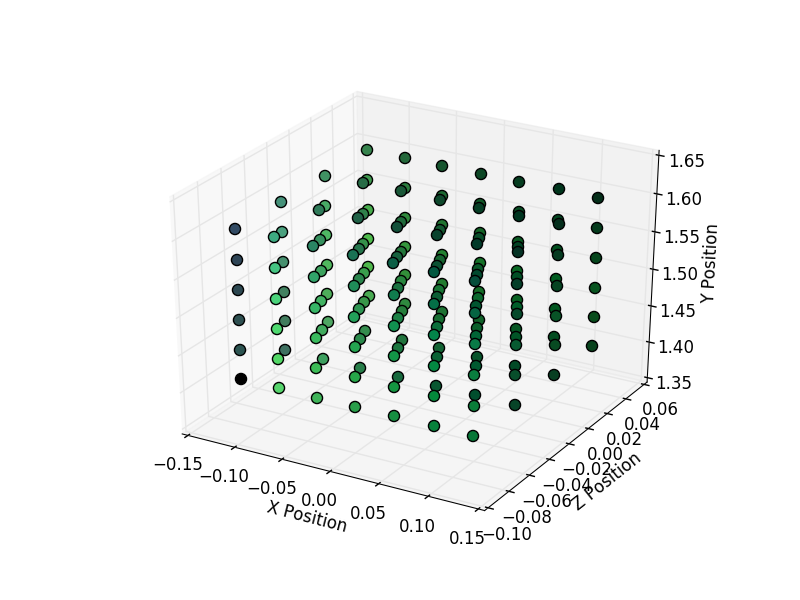
\includegraphics[width=4in]{images/K200000_global_dense_torque.png}
	\caption[A plot of a sample field for the torque based simulation]{Pictured above is a plot of instant linear acceleration samples at different pelvis positions within the balanced region.  Color indicates the magnitude, with the red, green, and blue channels corresponding to the x, y, and z components respectively of the acceleration sample.  Lighter color indicates a larger magnitude.  This is a clear example of the failures of this simulation method, as the samples seem to continuously increase from the one corner of the bounding box to the opposite diagonally, which does not produce a plausible animation as the character heavily favors one side, even with symmetric strengths.}
	\label{fig:torque_samples}
\end{figure}

Each iteration the error for the skeleton is calculated as for the samples but for the current state of the skeleton.  If the error is above the tolerance, a new position for the hip is calculated using proportional-derivative control, where the new position for the iteration of the controller, $u(i)$, is calculated as \[u(i) = k_p E_{all}(i - 1) + k_d(E_{all}(i-1) - E_{all}(i-2))\] where $i$ is the iteration, and $k_p$ and $k_d$ are weights which determine the rate of change.  The input to this PD controller is calculated by selecting a sample from the set of samples based on the acceleration error of the sample.  After filtering all plausible candidates from the samples, the candidate which minimizes balance error is selected and the vector between the current pelvis position and the sample pelvis position is given to the PD controller.  

The hip is repositioned based on the output of the PD controller, and the inverse kinematics component then iterates to calculate the positions of the remaining leg joints, assuming the feet should remain in the same position on the ground and the pelvis should remain at the chosen position.  This chooses a solution for the intervening joints.  At the next iteration, these new joint positions and angles are then used to compute the instant linear acceleration, center of mass, balance error, and acceleration error which are then passed back to the PD controller until the error in acceleration is below the tolerance.

%To determine which of numerous possible solutions is the most desirable, we take several samples. 


%\begin{figure}[ht]
%	\centering
%	\resizebox{\textwidth}{!}{
%		\begin{tikzpicture}[node distance = 0.5cm, auto]
% Bend Phase
    % before controller, need to calculate the desired 
    % place nodes
    \node [data, below of=path] (accel) {\nodebox{2.5cm}{Target Acceleration ($a$)}};
	\node [data, left=of accel] (mass) {\nodebox{3.5cm}{Body Mass assigned to each limb ($\left\lbrace m_0, \ldots, m_n\right\rbrace$)}};
    \node [stage, below= of accel] (forceCalc) {\nodebox{6cm}{Calculate desired force $F_{target} = \displaystyle\sum_{j=0}^n {m_j} a$}};
    % connecting lines
    \path [line] (accel) -- (forceCalc);
    \path [line] (mass) |- (forceCalc);
    % ----------------
	
    % PD controller
    % place nodes
    \node [substage, below=5cm of forceCalc] (bendErr) {Calculate error from desired force magnitude ($E_{force}$)};
    \node [substage, left=2.5cm of bendErr] (bendBal) {Calculate balance error ($E_{balance}$)};
    \node [substage, above=1cm of bendBal] (comCalc) {\nodebox{5cm}{Calculate Center of Mass \[C_{mass} = \displaystyle\sum_{\forall m} m \cdot position(m)\]}};
    \node [data, below left=1cm and -2cm of bendErr] (bendErrAll) {\nodebox{4cm}{$E_{all} = E_{force} + E_{balance}$}};
    \node [decision, below=0.5cm of bendErrAll] (bendPDTest) {$E_{all} \overset{?}{\le} \epsilon$};
    \node [substage, left=1cm of bendPDTest] (bendPDEq) {Set new hip position based on $u(i) = k_p E_{all}(i-1) + k_d \left(E_{all}(i-1) - E_{all}(i-2)\right)$};
    \node [stage, label={[shift={(-0.5cm, 2cm)}, rotate=90]180:\LARGE PD Controller}, fit=(comCalc) (bendErr) (bendBal) (bendErrAll) (bendPDEq) (bendPDTest)] (bendPD) {};
    \node [data, below=2cm of bendPDTest] (bentSkel) {\nodebox{3cm}{Skeleton in bent position ($\theta_{x} \forall x \in J_m$)}};
    \node [data, below=1cm of bendPDEq] (bendPDConst) {
    \nodebox{4cm}{Proportional and Derivative weights ($k_p, k_d$)}};
    % connecting lines
	\path [line] (forceCalc) -- (bendErr);
	\path [line] (comCalc) -- (bendBal);
	\path [line] (bendErr) |- (bendErrAll);
    \path [line] (bendBal) |- (bendErrAll);
    \path [line] (bendErrAll) -- (bendPDTest);
    \path [line] (bendPDTest) -- (bendPDEq);
    \path [line] (bendPDTest) -- (bentSkel);
    \path [line] (bendPDConst) -- (bendPDEq);
    % ----------------
    
    % CoM inputs
    % place nodes
    \node [data, above =2cm of comCalc] (skeleton) {\nodebox{2.5cm}{Model with skeleton attached ($J = \left\lbrace j_0, \ldots, j_n \right\rbrace$, contains at least a pelvis and both left and right hips, knees, ankles, heels, and toes)}}; 
    \node [data, left=1cm of skeleton] (mjoints){\nodebox{3cm}{Muscled joints ($J_m = \lbrace$ $j_{pelvis}$, $j_{Lhip}$, $j_{Rhip}$, $j_{Lknee}$, $j_{Rknee}$, $j_{Lankle}$, $j_{Rankle}$, $j_{Lheel}$, $j_{Rheel}$, $j_{Ltoe}$, $j_{Rtoe}$ $\rbrace$}};
    \node [data, left=1cm of mjoints] (muscles) {\nodebox{3cm}{Muscle spring constant for muscled joints ($\left\lbrace k_0, \ldots, k_11\right\rbrace$)}};
	\node [data, left=1cm of muscles] (jconst) {\nodebox{2cm}{Rotation constraints for joints ($\theta_{min}, \theta_{max}$ $\forall j \in J_{muscled}$)}};
	
	% connecting lines
	\path [line] (skeleton) -- (comCalc);
	\path [line] (mjoints) -- ++(0cm, -3.4cm) -| (comCalc);
	\path [line] (muscles) -- ++(0cm, -3.5cm) -| (comCalc);
	\path [line] (jconst) -- ++(0cm, -3.6cm) -| (comCalc);
	% ----------------	
	
	% IK solver side stage
	% place nodes
	\node [data, left=3cmof bendPDEq] (IKCurJoint) {\nodebox{4cm}{$R = position(j)$ $\forall j \in J_{ik} \subseteq J$ starting with the root (hip joint).}};
	\node [data, left=1cm of IKCurJoint] (IKTargetPos) {\nodebox{4cm}{Target position for joint, in this case keeping $E$ in it's original position ($D$).}};
	\node [data, left=1cm of IKTargetPos] (IKEndJoint) {\nodebox{2cm}{Joint to move to target ($E$).}};
	\node [data, above=1cm of IKEndJoint] (IKRE) {\nodebox{3cm}{Normalized vector $\vec{RE}$}};
	\node [data] (IKRD) at (IKCurJoint |- IKRE) {\nodebox{3cm}{Normalized vector $\vec{RD}$}};
`	\node [substage, above=2cm of IKTargetPos] (IKEq) {$\theta_j = \vec{RD} \times \vec{RE}$.};
	\node [data, above left=1cm of IKEq] (IKItrs) {\nodebox{3cm}{Number of iterations for IK solver ($num_itr$)}};
	\node [data] (IKPartBent) at (IKEq |- comCalc) {\nodebox{2cm}{Bent skeleton reflecting $u(i)$.}};
	\node [stage, label={[shift={(-0.5cm, 1.5cm)}, rotate=90]180:\LARGE IK Solver}, fit=(IKCurJoint) (IKEndJoint) (IKTargetPos) (IKItrs) (IKRD) (IKEq) (IKPartBent)] (bendIK) {Requires joints to be in a single chain.};
    % connecting lines
    \path [line] (bendPDEq) -- (IKCurJoint);
    \path [line] (IKPartBent) -| ++(6cm, -1.6cm) -| (bendErr);
    \path [line] (IKPartBent) -- (comCalc);
    \path [line] (IKCurJoint) -- (IKRD);
    \path [line] (IKEndJoint) -- (IKRE);
    \path [line] (IKTargetPos) |- (IKRD);
    \path [line] (IKTargetPos) |- (IKRE);
    \path [line] (IKRD) |- (IKEq);
    \path [line] (IKRE) |- (IKEq);
    \path [line] (IKEq) -- (IKPartBent);
    \path [line] (IKItrs) |- (IKEq);
    % ----------------
\end{tikzpicture}
%	}
%	\caption[Diagram of windup phase algorithm]{Algorithm diagram of the windup phase.}
%	\label{fig:bendPhase}
%	%TODO decision lines need to be labeled
%\end{figure}

%\begin{table}[ht]
%	\centering
%	\caption[Table of PD controller constants for windup phase]{Example values for the PD controller constants, showing the sweet spot that we use as well as the effect of going higher or lower (how do we show this effect, show that the steps are too large or too small? time or iterations to finish?).}
%	\label{tab:windup_pd_vals}
%\end{table}

%\subsubsection{Force calculation}
%TODO force calculation should be done with error in net torque instead of error in force as we don't really have a resultant force here and the net force really means nothing
% calculation of the muscle flexion

%Current force is computed by approximating muscles as linear springs attached to two bones and crossing a joint.  The change in spring length is produced by the bend of the joint which opens a space between the rigid bones that the spring must stretch across.  This approximation uses spring constants that simulate a flexed muscle that has been stretched by an amount equal to \[\theta = cos^{-1} \left( \dfrac{2 k^2 r^2}{F^2} - 1 \right)\] which requires a more rigid spring constant.  In this equation, $r$, represents the width of the bone, which is a constant that changes the amount the character must bend to achieve a force.  This acts similarly to the $k$ value, which represents the stiffness of the spring, or a constant for the linear restoring force of the muscle.  
%TODO For our simulations, we used values in the range ().
%TODO values and equation
%TODO tables of values with varied k and varied r and corresponding bend/angle
%\begin{table}[ht]
%	\centering
%	\caption[Table of spring muscle constants]{A table of various values for k and r, demonstrating effect on the model's bend.  TODO Columns of k and r (varied individually), and image of fully bent character resulting from values.}
%	\label{tab:variedSpringValues}
%\end{table}

%At each iteration of the PD controller, current force output of the legs is computed.  An accurate calculation of the force must take into account the torques ($\vec{\tau}$) produced by the muscles on each joint.  We use a simplified version, calculating the magnitudes of the torques which avoids the complexity of implementation and computation.  This is found for a joint j as \[\tau_j = ||\vec{r_j}|| F_j\] where r is the moment arm, the cross product between the vector between the attachment point of muscle and the center of the joint with the direction of the muscle crossing the joint.  Direction of a muscle is in the direction of restoration of the spring (TODO double check this, is this always the value we want, point placed along the spring based on the masses on each end) as used in \cite{muscle_based_bipeds}.
%TODO does this setup effectively result in springs connected in series? No because you can assume that the muscles you don't want to unbend with remain rigid?
%TODO does this give a sort of impulse function as you unbend at the hips and knees, then the ankles?
%TODO this is where the torques come into play, and they're absolutely necessary

%\begin{figure}[ht]
%	\centering
%	\caption[Algorithm diagram for calculation of force error]{Force error calculation}
%	\label{fig:forceErr}
%\end{figure}

%To calculate the error used for PD control, the vector between the two forces is measured, indicating the change required in both direction and magnitude.  As we require the force to act in the direction of acceleration, the main adjustment is the force magnitude.  When instead considering the torque magnitude, the magnitude alone can be considered. (TODO I think I need to be using the torque magnitude instead of a force here).


\subsection{Thrust and Takeoff}
\label{subsection:thrust}
Upward acceleration is animated by calculating the angular accelerations of the joints given the forces acting upon them and the resulting torques.  Torque is the change in angular momentum over time, allowing for the acceleration to be calculated as the mass can be assumed to be constant: \[\tau = \dfrac{dL}{dt} = m \dfrac{dv_{\theta}}{dt} = m a_{\theta}\] where $\tau$ is the torque of a joint, $L$ is the angular momentum, $m$ is the mass of the limb, which must take into account the mass of the rest of the body which is also moved by the limb, $v_{\theta}$ is the angular velocity and $a_{\theta}$ is the angular acceleration. This results in the below equation for determining angular acceleration. \[a_{\theta} = \dfrac{\tau}{m}\]

Using angular acceleration, the intermediary poses for the model can be determined at each time step.   For each frame, an explicit Euler integration is performed to determine first angular velocity and finally angle.  As the character continues to extend, a check is made for if the character has yet reached full extension as described in \ref{subsection:skel_joints}.  At full extension, the character can no longer accelerate in the direction of the jump, and the character breaks contact with the ground to enter the in-air phase.

As the windup phase of the torque based simulation fails, it is difficult to quantify or qualify the success and failure of this portion of the simulation.  For values where the simulation could not complete the windup phase, the in-air portion is unavailable and for values where the windup phase completes, the values are erratic and fail to produce valid poses, often resulting in extreme contortions of the model.

%To select the minimum sample, the collected data were organized first by the difference between the linear momentum calculated and the desired linear momentum, and the top ten percent were selected.  Ten percent was found empirically to be a good selection of points to select the most balanced from while also retrieving points with very low differences from the desired.

%\subsection{Rebalancing}
%As the character re-positions its pelvis, the balance must be calculated again and its position accordingly re-adjusted.  To maintain the position of the legs, we use the upper body to achieve balance.  A separate PD controller is used to regulate the rate of movement.  While the character shifts its balance to achieve a particular acceleration, it bends its upper body, moving the weight forward, backward, left, or right to attempt to center itself over its supporting polygon.

%%%%%%%%%%%%%%%%%%%%%%%%%%%%%%%%%%%%%%%
%               Energy                %
%%%%%%%%%%%%%%%%%%%%%%%%%%%%%%%%%%%%%%%
\section{Energy Based Calculation}
Another way we simulated jumping motions was energy based.  We assumed that the kinetic energy of the character traveling at a calculated velocity from its start position to the destination position is equivalent to the summed elastic potential energies of the leg muscles.  The direction of the velocity is determined by the direction the center of mass is accelerated after the windup phase, and we assume that this is achievable given that the character can achieve the desired energy.  

Change in direction is accomplished through usage of the feet and shift of weight during the acceleration and windup phases, applied through balance and inverse kinematic calculations.  If a character wishes to move forward, they shift their weight back farther during windup, allowing them to accelerate forward farther before becoming airborne.  In the same way, shifting to one side can allow the character to accelerate in the opposite direction for non-forward jumps.  As with the torque-based simulation, the jump follows the stages of path estimation, windup, thrust, in-air, and landing.

\subsection{Path Estimation and Windup}
\label{subsection:energy_path}
Kinetic energy is calculated as \[ E_k = \frac{1}{2} m v^2 \] where $m$ is the mass of the character and $v$ is the velocity.  Mass is a constant specified by the user, and we calculate the desired velocity and acceleration as in the torque based path estimation as described in section \ref{subsection:torque_path}.  Instead of 

Like with the torque-based method, we took samples in the region where the character maintains balance as in \ref{subsubsection:torque_sample}.  Samples were collected at regular intervals within a bounding box defined by the character's supporting polygon, the ground, and the the height of the character's pelvis at full extension.  The pelvis was repositioned and the resulting elastic potential energy measured.  Candidate samples were selected by finding all samples with \[ E_{kinetic} - E_{elastic} \le \epsilon(E_kinetic)\] and the candidate with the lowest incurred balance error was selected.

\begin{figure}[ht]
	\centering
	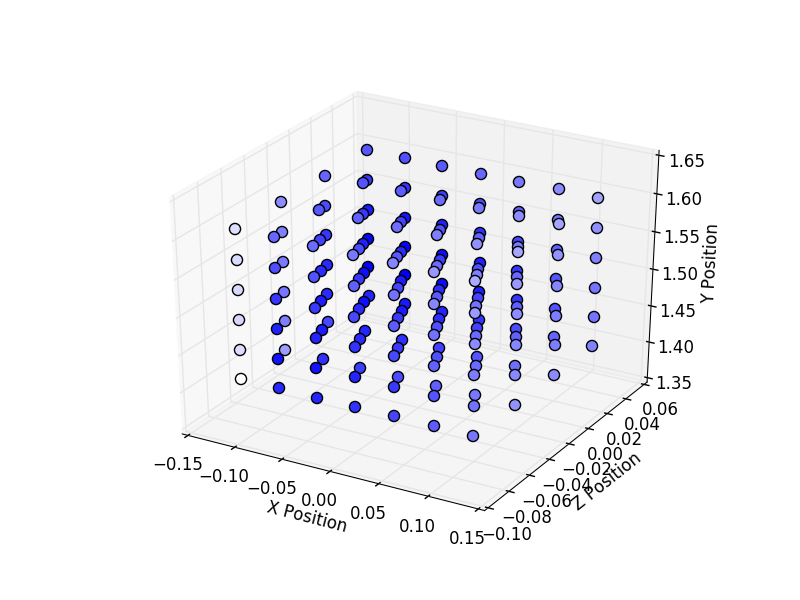
\includegraphics[width=4in]{images/K200000_global_dense.png}
	\caption[A plot of a sample field for energy based simulation]{A graph of samples for the character with all muscle k values set to $200000$.  The pelvis positions are plotted, with the color of the data point indicating the energy.  A darker point indicates a higher total elastic energy calculated for the skeleton when the pelvis is positioned at that point.}
	\label{fig:energy_samples}
\end{figure}

Our sampling method does not guarantee an optimal solution, but can be seen as guaranteeing an approximate minimum.  We choose a sample with minimum balance error and iteratively approach it, which greedily finds the nearest sample to the rest pose which satisfies the energy equivalence, $E_{kinetic} = \displaystyle\sum E_{elastic}$.  While not guaranteed to be the minimum, this guarantees that we find a near-minimum value assuming the region is continuous.  Figure \ref{fig:energy_samples} is a graph of samples for a particular run with all muscle $k$ values set to 200000.  Color indicates the calculated energy for the sample point, with higher saturation of blue indicating a higher energy value for the sample.  The higher energy samples tend to be clustered towards the center of the sample group, which meets expectations as most humans will bend to a position such that their hip is between its normal position when standing and the level of their knees.

%Given that work is the change in kinetic energy, velocity
%\begin{align*}
%	W &= F d \\
%	&= \delta E \\
%	&= \frac{1}{2} m \left(v^2 - v_0^2\right)
%\end{align*}

\subsection{Solutions to the Energy Assignment Problem}
\label{subsection:energy_prob}
The setup of the problem resembles a quadratic programming problem.  In this problem, we minimize: \[ \vec{x}^T \mathbf{Q} \vec{x} \] subject to
\[ \vec{x}^T \mathbf{P} \vec{x} \le r \] where $x \in R^6$ and $\mathbf{Q}$ and $\mathbf{P}$ are square, $6 \times 6$ matrices.  $\mathbf{Q}$ for our problem is a diagonal matrix, where the diagonals contain the spring constants $\left\lbrace k_1, k_2, ... , k_6 \right\rbrace$ and $\mathbf{P}$ is $- \mathbf{Q}$.  We can introduce additional constraints in the form of maximum and minimum values for all $x_i \in \vec{x}$, where the minimum and maximum are calculated at the minimum and maximum rotations of the joint, producing the extremes in spring displacement.

This problem of quadratically constrained quadratic programming is NP-hard and as such we sought a simpler problem or approximation to solve to obtain a solution.  As with the torque method, we choose a sampling-based approach as there is a known limit on the possible solutions in our case: balance.  

\subsection{Thrust, In Air, and Landing}
\label{subsection:energy_thrust}
Thrust for the energy based simulation works off of explicit euler integration.  The calculated acceleration from the path estimation stage is used to accelerate the character over the duration of $t_{windup}$.  At each time step, the pelvis is translated by $v_{takeoff}$, which begins at 0 and gains $\vec{a} dt$ per frame.  Each frame the character's extension is checked using the function described in \ref{subsection:skel_joints}, and when it falls below a tolerance of $0.1$, the character is considered fully extended and the in air phase begins.  During the thrust, the movement can sometimes proceed faster than the IK solver can converge, so we pause the simulation briefly and only iterate the solver until it converges.

The in air phase proceeds similarly, with the character translated by the calculated velocity from the path estimate each frame.  Velocity is modified by $\vec{g} dt$ where $\vec{g}$ is the acceleration due to gravity, resulting in the desired parabolic path of the player through the air.  Ray casts are performed to check if the character's feet have contacted a surface to land on.  These ray casts are made from above toe, heel, and middle of the foot, starting above and passing through the points to produce a longer ray for more stable results.  Once one of these ray casts indicates the feet have touched such a surface, the character enters the landing phase.

A landing controller is beyond the scope of this thesis, and thus we end the simulation as the character's feet touch a suitable surface.  As described in Chapter \ref{chapter:previous_work}, other controllers can be composed with this controller to produce a full animation, handling the complexities of the landing motion as a separate, modular controller.

\section{Summary}
\label{subsection:animation_summary}
The character is modeled as a mesh with a skeleton and muscles.   The skeleton was created as a tree of joints with the root at the hip.  Muscles were placed along the limbs, crossing a single joint and anchored to the bones on either side.  Force and energy outputs of the muscles were calculated as linear springs, with spring displacements calculated from the angle of the joint.  An inverse kinematic solver was used to aid in creating poses.

Two methods were used for the simulation, one using torque based calculations and the other using energy based calculations.  Each method proceeded through the stages of path estimate, windup, thrust, in air, and landing, with similar calculations used to produce an error function to quantify character poses.  In the torque based simulation, error was calculated by using the muscles to calculate torques, and from the torques accelerations.  In the energy based simulation, error was calculated as the difference between elastic potential energy and target kinetic energy.  

Samples were collected using these error functions, with the selected best sample minimizing both the balance error and either the acceleration or energy errors for the torque and energy simulations respectively.  A PD controller iteratively moved the character's pelvis position towards the selected sample until the error between the calculated values for the frame and the desired values were below a tolerance.  After the character moved its pelvis to the chosen sample position to reduce the error below tolerance, it performed the thrust and in air portions of the jump treated as a rigid body, with the simulation ending when the character's feet touch the ground.